\documentclass[fleqn, xcolor=x11names]{beamer}
\usetheme{Frankfurt} % шаблон
\usecolortheme{default} % цветовая схема
\usepackage[11pt]{moresize}
\usepackage{multimedia}
\usepackage[T1]{fontenc}
\usepackage{pgfplots}
\usepackage[utf8]{inputenc}
\usepackage[russian]{babel}
\usepackage{media9}
\usepackage{listings}
\usepackage{amsmath}
\usepackage{color}
\usepackage{parskip}
\usepackage{wrapfig}

\usepackage{graphicx}
\lstdefinestyle{myLatexStyle}{
    basicstyle=\small\ttfamily,
    language={python},
    numbersep=5mm, numbers=left, numberstyle=\tiny, % number style
    breaklines=true,frame=single,framexleftmargin=8mm, xleftmargin=8mm,
    backgroundcolor=\color{green!5}, frameround=fttt,escapeinside=??,
    rulecolor=\color{red},
    morekeywords={% Give keywords here
        numpy},
    keywordstyle=\color[rgb]{0,0,1},                    % keywords
        commentstyle=\color[rgb]{0.133,0.545,0.133},    % comments
        stringstyle=\color[rgb]{0.627,0.126,0.941}  % strings
}
\lstset{style=myLatexStyle}

\setbeamertemplate{navigation symbols}{}
\setbeamertemplate{footline}{%
    \hspace{0.99\paperwidth}%
    \usebeamerfont{title in head/foot}%
    \insertframenumber\,/\,\inserttotalframenumber%
}



\title{Meta-learning}
\author[Медведев~Д.\,В.]{Медведев Алексей Владимирович}
\institute[ВМК МГУ]{МГУ имени М. В. Ломоносова,
факультет ВМК, кафедра ММП}
\date{} 

\begin{document}

\begin{frame}
\maketitle
\end{frame}

\begin{frame}
\begin{block}{Meta-learning}
\begin{itemize}

\item Построение системы для улучшения работы модели с конкретной задачей (подбор оптимальных гиперпараметров черного ящика).

\item Адаптация алгоритма для решения новых задач.

\item Аналогия "--- эволюционный процесс, создавший человеческий мозг.
\end{itemize}
\end{block}
\end{frame}



\begin{frame}[fragile]\frametitle{Neural Architecture Search}
{\footnotesize

\begin{figure}[h]
\begin{center}
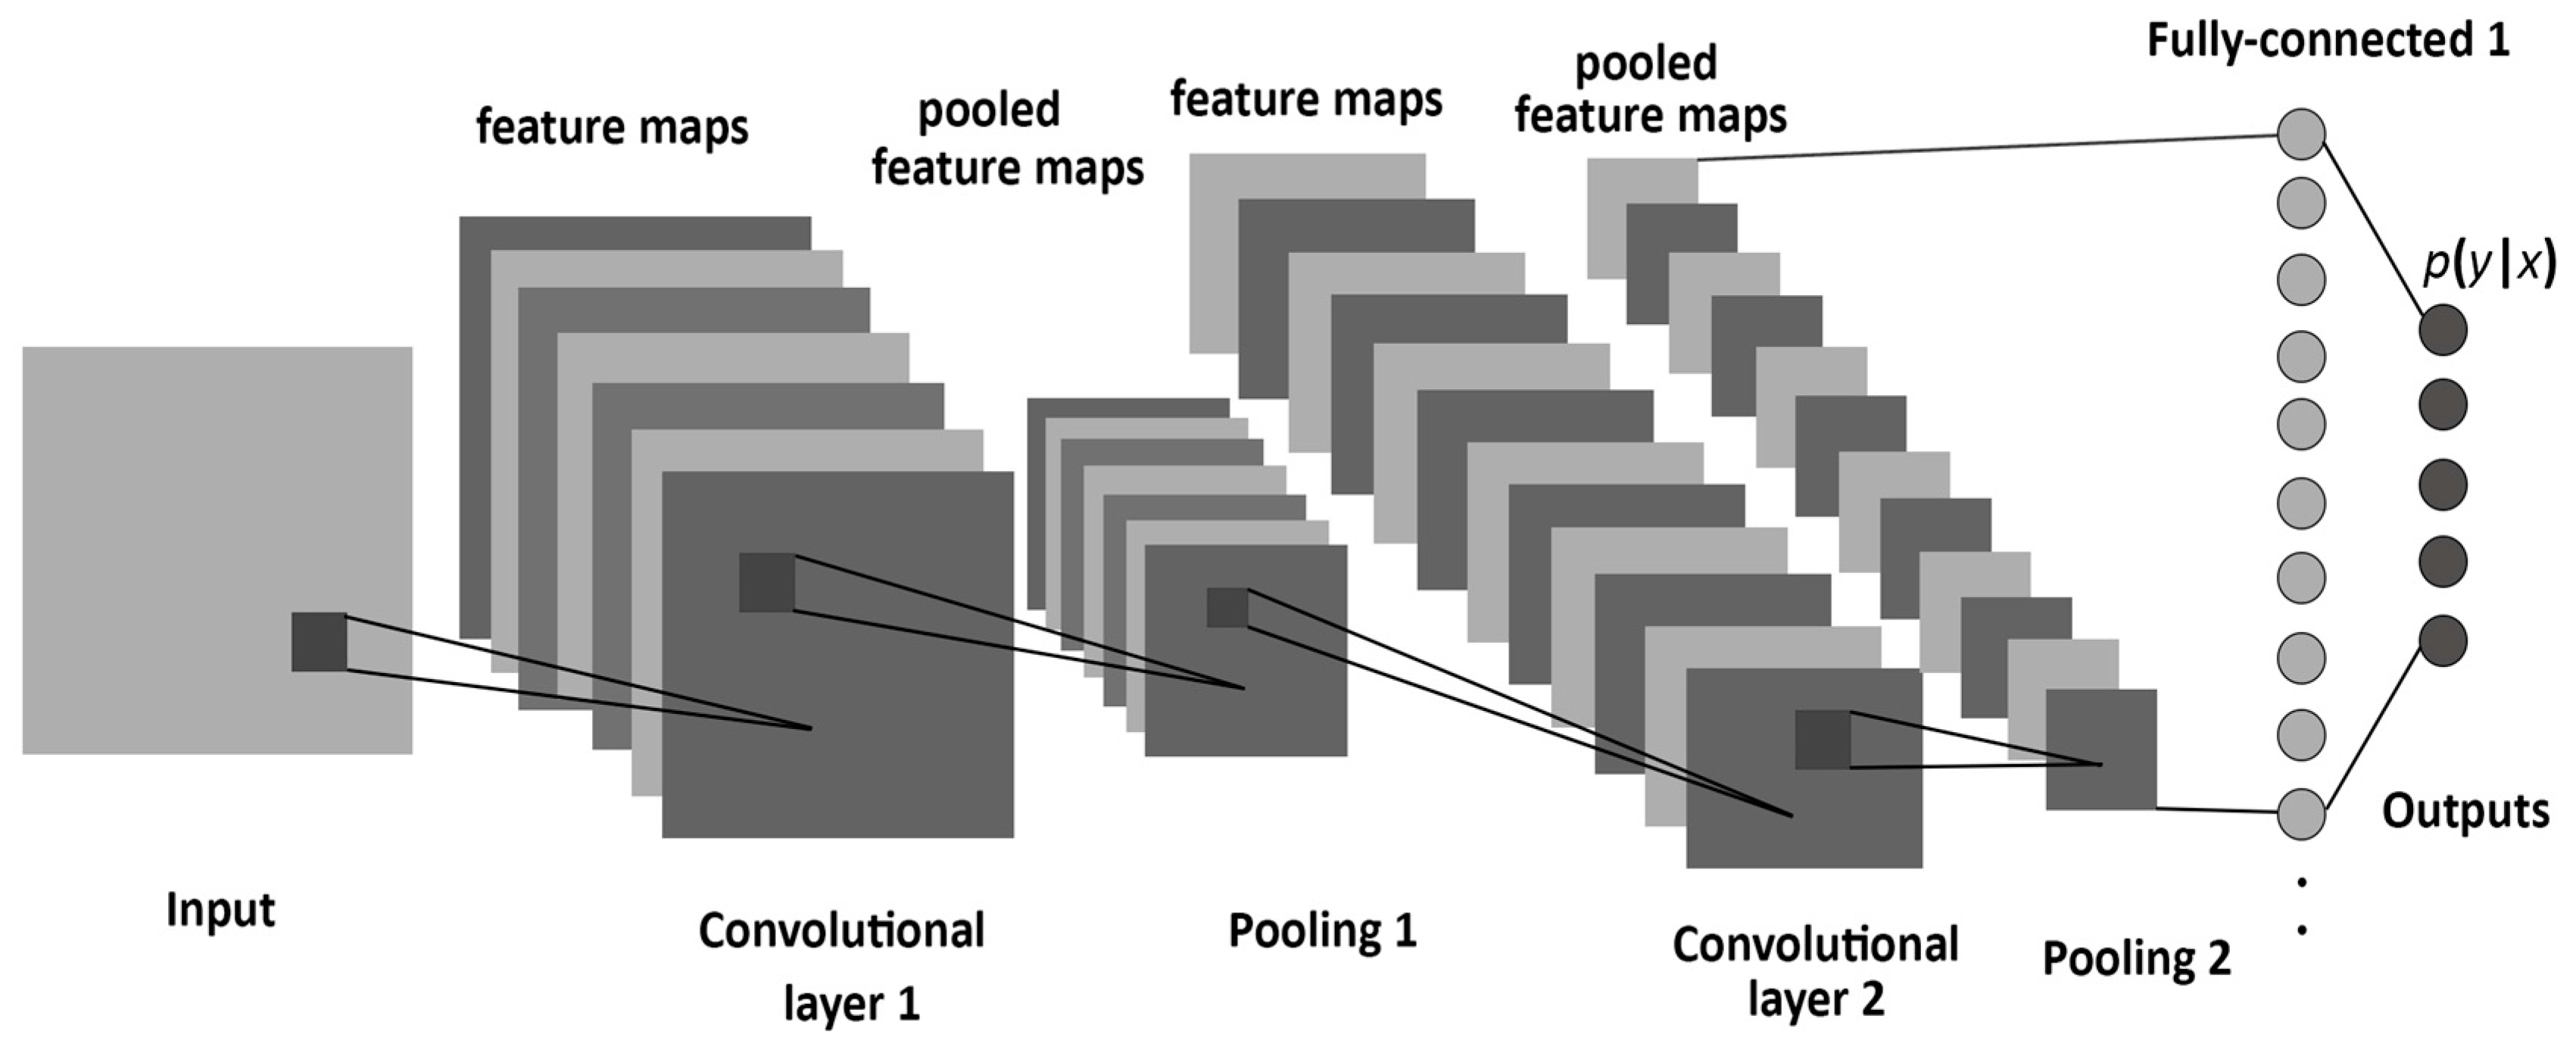
\includegraphics[scale=0.5]{/home/alex/python/D'yakonov/convnet.png}
\end{center}
\end{figure}

\begin{block}{Проблема}
Нейронные сети хорошо показали себя в задачах обработки изображений, речи, понимания языка. Конструирование нейросети остается непростой задачей, требующей определенных навыков.

\end{block}

\begin{block}{Идея}
Создать алгоритм, который сможет описывать архитектуру нейросети для данной задачи машинного обучения.

\end{block}



}
\end{frame}

\begin{frame}[fragile]\frametitle{Neural Architecture Search}

\begin{block}{Neural Architecture Search [Barret Zoph, Quoc V. Le 2017]}

\begin{itemize}
\item Архитектура нейросети может быть записана как строка произвольной длины

\item Можно взять RNN (controller), каждый блок которой будет отвечать за определенный параметр искомой архитектуры(Количество фильтров в слое сверточной нейросети, с какими слоями соединен данный слой(skip connections) и т.д.)

\item Обучить controller с помощью reinforcement-learning, считая что вознаграждение это точность полученной архитектуры на кросс-валидации
\end{itemize}

\end{block}


\end{frame}

\begin{frame}\frametitle{Neural Architecture Search}

\begin{figure}[h]
\begin{center}
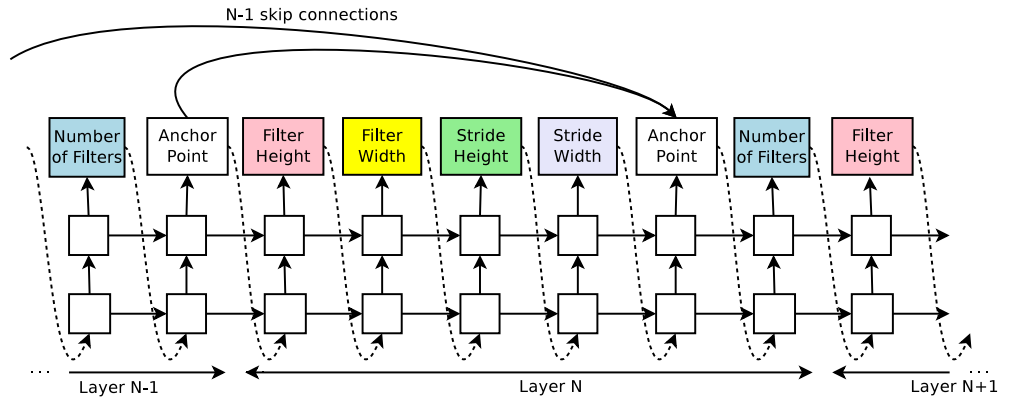
\includegraphics[scale=0.35]{/home/alex/python/D'yakonov/nas_architecture.png}
\end{center}
\end{figure}
{\footnotesize
\begin{itemize}
\item сontroller представляет собой RNN
\item каждый выход --- softmax
\item каждый блок предсказывает свой параметр конструируемой архитектуры
\item блоки сгруппированы по слоям
\end{itemize}
}
\end{frame}

\begin{frame}\frametitle{Neural Architecture Search}



\begin{figure}[h]
\begin{center}
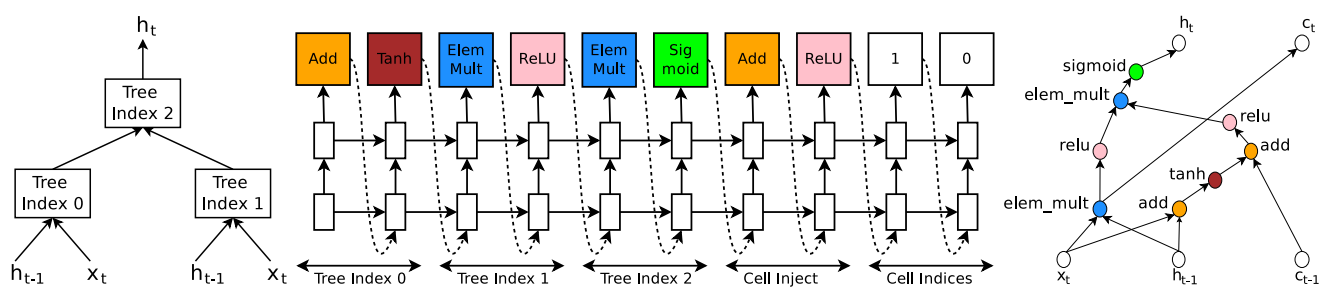
\includegraphics[scale=0.3]{/home/alex/python/D'yakonov/nas_rnn_architecture.png}
{\footnotesize
\caption{Пример архитектуры controller'a, для рекуррентной нейросети.}
}
\end{center}
\end{figure}


\end{frame}



\begin{frame}[fragile]\frametitle{Reinforcement Learning}
\normalsize


\begin{minipage}[t]{.5\textwidth}
{\footnotesize
Введем некоторые обозначения:
\begin{itemize}
\item a "--- действие.
\item s "--- состояние.
\item $\pi$ "--- стратегия $p(a|s)$.
\item $r_{t}$ "--- вознаграждение.
\item задача максимизировать:
\begin{center}
$J(\theta) = E_{\pi_{\theta}} [\sum \limits_t r_t]$
\end{center}
\end{itemize}
}
\end{minipage}
\begin{minipage}[t]{.3\textwidth}
\begin{center}

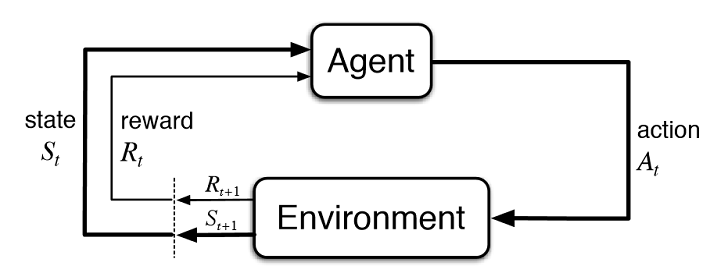
\includegraphics[scale=0.28]{/home/alex/python/D'yakonov/RL1.png}


\end{center}
\end{minipage}\qquad
\end{frame}

\begin{frame}[fragile]\frametitle{Reinforcement Learning}
{\footnotesize
\begin{block}{Policy gradient}
\begin{itemize}
\item Оптимизация $\pi_{\theta}$ напрямую
\item Градиент функционала: $\nabla_{\theta}J(\theta) = \sum \limits_{\tau} R(\tau)P(\tau, \theta) \nabla_{\theta} \log P(\tau, \theta)$
\begin{center}
$\nabla_{\theta}J(\theta) = \sum \limits_{\tau} R(\tau) \nabla_{\theta}P(\tau, \theta) = \sum \limits_{\tau} R(\tau)P(\tau, \theta) \frac{\nabla_{\theta}P(\tau, \theta)}{P(\tau, \theta)} =  \sum \limits_{\tau} R(\tau)P(\tau, \theta) \nabla_{\theta} \log P(\tau, \theta) $
\end{center}
\item Где: $ P(\tau, \theta) = \prod \limits_{t=0}^{H} P(s_{t+1}|a_t,s_t) \pi_{\theta}(a_t|s_t)$

\item Несмещенная оценка: $\nabla_{\theta}J(\theta) \approx \frac{1}{m}\sum \limits_{i=1}^m R(\tau^i)\nabla_{\theta} \log P(\tau^i, \theta)$

\item Не зависит от динамики среды: 
\begin{center}
$\nabla_{\theta} \log P(\tau, \theta) = \nabla_{\theta} \log \left(\prod \limits_{t=0}^{H} P(s_{t+1}|a_t,s_t)\pi_{\theta}(a_t|s_t)\right) = \sum \limits_{t=0}^{H} \nabla_{\theta} \log \pi_{\theta}(a_t|s_t)$
\end{center}

\end{itemize}

\end{block}
}
\end{frame}

\begin{frame}[fragile]\frametitle{REINFORCE}

{\footnotesize
\begin{block}{REINFORCE algorithms [Williams, 1992]}

\begin{itemize}
\item Оценка градиента хоть и несмещенная, но может имет большой разброс.
\item Чем больше $R(\tau)$ тем разброс больше:

Пусть $\log \pi_{\theta}(\tau) = [0.5,0.2,0.3]$, и $R(\tau) = [1000,1001,1002]$,

тогда $Var(0.5 \cdot 1000,0.2 \cdot 1001,0.3 \cdot 1002) = 23286.8$.
 
Если $R(\tau) = [1,0,-1]$, то $Var = 0.1633$.
\item  Тогда оценка градиента принимает следующий вид:
\begin{center}
$\nabla_{\theta}J(\theta) \approx \frac{1}{m}\sum \limits_{i=1}^m \nabla_{\theta} \log P(\tau^i, \theta) (R(\tau^i) - b)$
\end{center}
\item Доказательство несмещенности:
\begin{center}
$   E_{\pi_{\theta}} \left[\nabla_{\theta} \log P(\tau, \theta)b \right] =  \sum \limits_{\tau} P(\tau, \theta) \nabla_{\theta} \log P(\tau, \theta)b = \sum \limits_{\tau} \nabla_{\theta}P(\tau, \theta)b = b \nabla_{\theta} \sum \limits_{\tau} P(\tau) = b \times 0$
\end{center}

\end{itemize} 
\end{block}
}
\end{frame}


\begin{frame}[fragile]\frametitle{Neural Architecture Search}

\begin{figure}[h]
\begin{center}
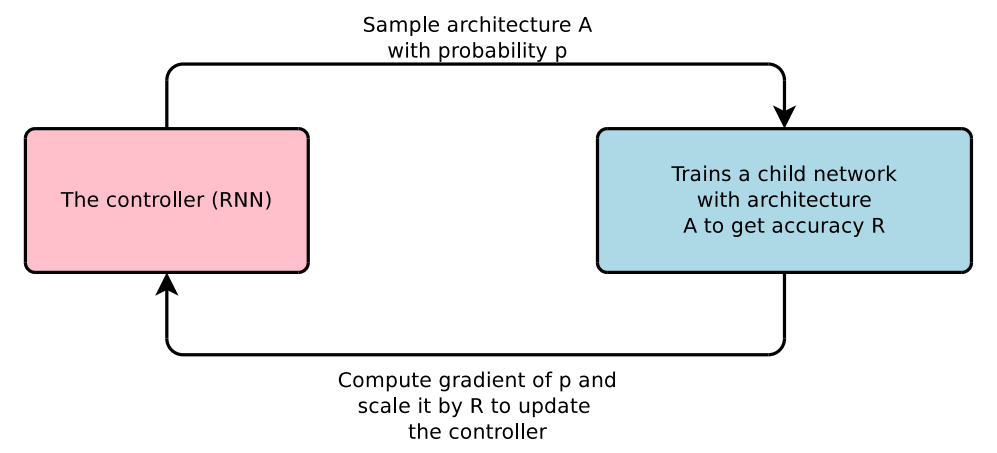
\includegraphics[scale=0.3]{/home/alex/python/D'yakonov/nas_scheme.png}
\end{center}
\end{figure}

{\footnotesize

\begin{itemize}

\item Градиент функционала принимает следующий вид:
\begin{center}
$ \nabla_{\theta_c} J(\theta_c) = \frac{1}{m}\sum \limits_{k=1}^m  \sum \limits_{t=1}^T \nabla_{\theta_c} \log{P(a_t | a_{(t-1):1}; \theta_c)}(R_k-b)$
\end{center}

\item $m$ --- размер batch'a, созданных controller'ом архитектур, 

\item $R_k$ --- вознаграждение, которое получено для данной архитектуры, 

\item $T$ --- количество гиперпараметров, которые controller должен определить,

\item $P$ --- вероятностная модель, которую моделирует controller.
\end{itemize} 
}


\end{frame}





\begin{frame}\frametitle{Neural Architecture Search}

\begin{figure}[h]
\begin{center}
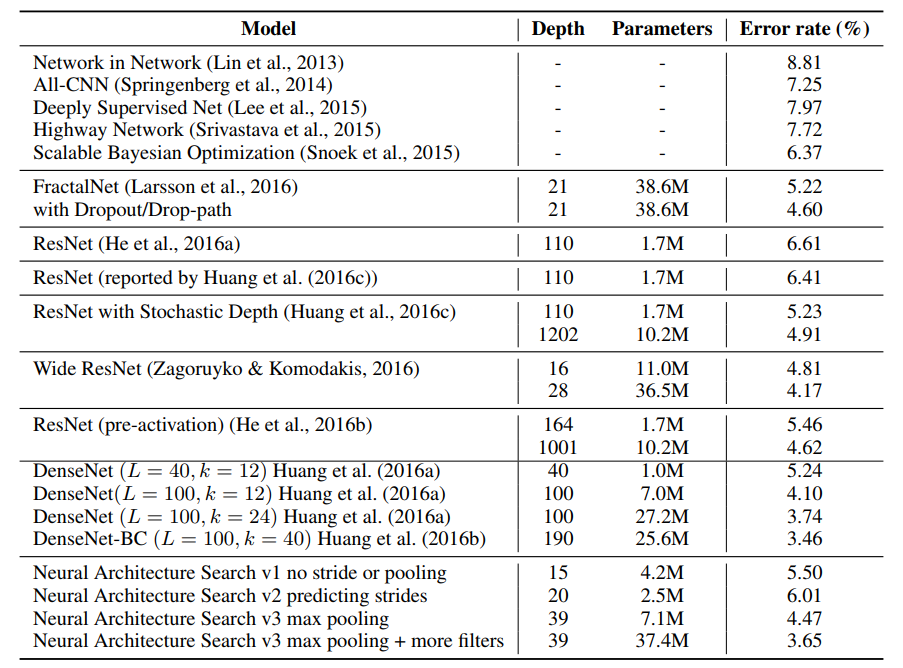
\includegraphics[scale=0.35]{/home/alex/python/D'yakonov/nas_cifar10.png}
\caption{Результаты state-of-the-art моделей и найденных алгоритмом архитектур на датасете CIFAR10(классификация).}
\end{center}
\end{figure}

\end{frame}


\begin{frame}\frametitle{Neural Architecture Search}

\begin{figure}[h]
\begin{center}
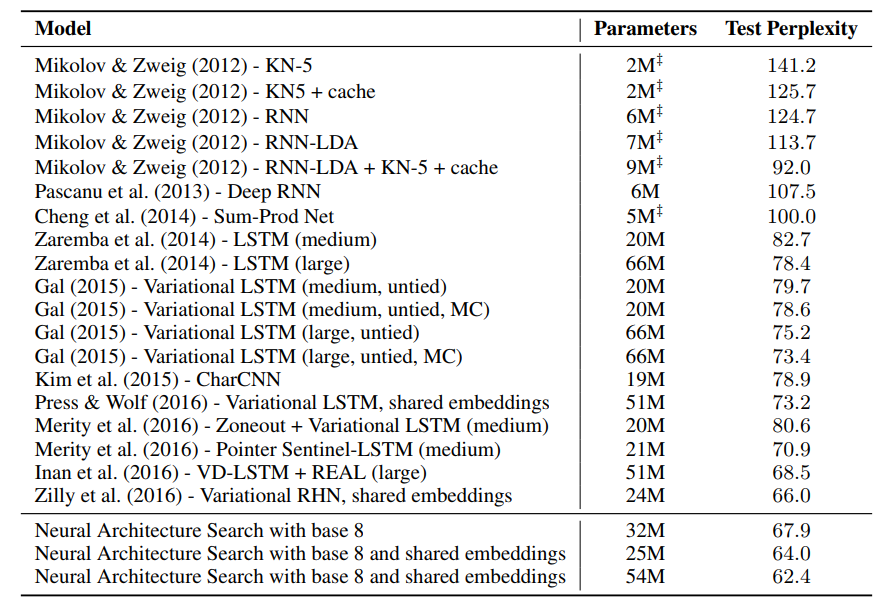
\includegraphics[scale=0.35]{/home/alex/python/D'yakonov/nas_ptb.png}
\caption{Результаты state-of-the-art моделей и найденных алгоритмом архитектур на датасете  Penn Treebank.}
\end{center}
\end{figure}

\end{frame}

\begin{frame}\frametitle{Neural Architecture Search}




\begin{block}{Результат}
{\footnotesize Алгоритм нашел несколько интересных архитектур как в случае классификации, так и в случае более сложной задачи моделирования языка. Более того последние показали еще и хорошие результаты на задаче машинного перевода.}
\end{block}

\begin{table}[h]
\begin{center}
\begin{tabular}{*{3}{c}}

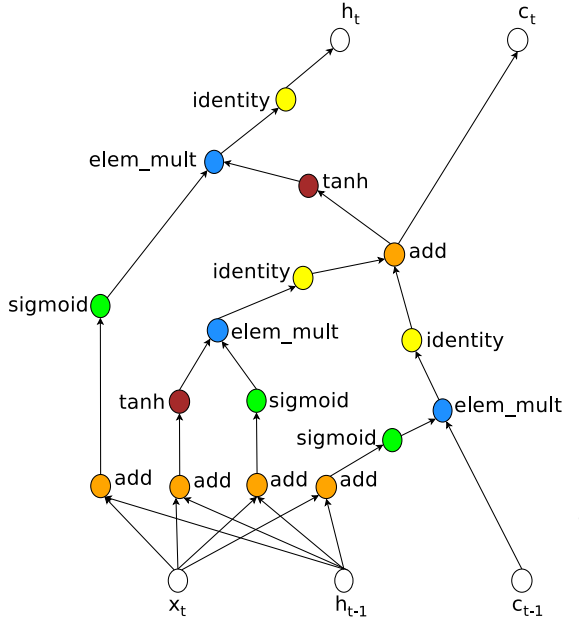
\includegraphics[width = 3cm]{/home/alex/python/D'yakonov/nas_lstm.png} &
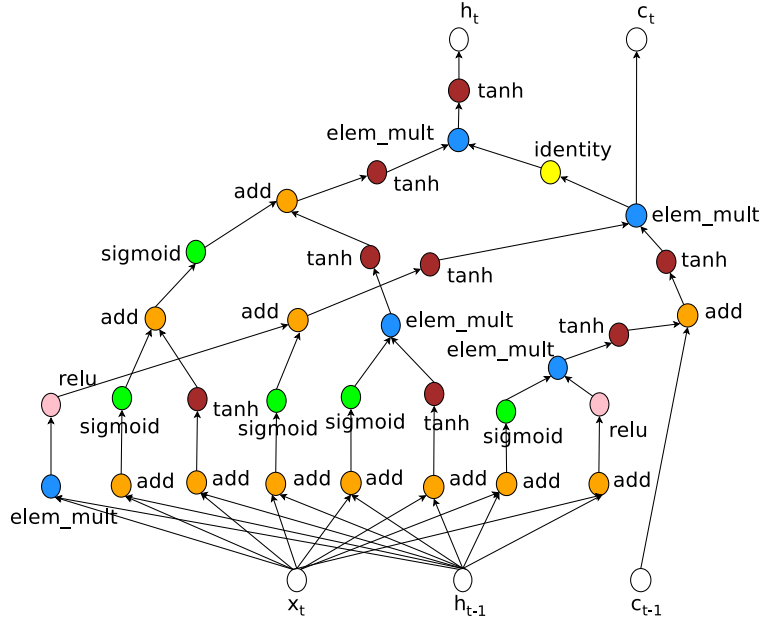
\includegraphics[width = 3cm]{/home/alex/python/D'yakonov/nas_new_cell.png} &
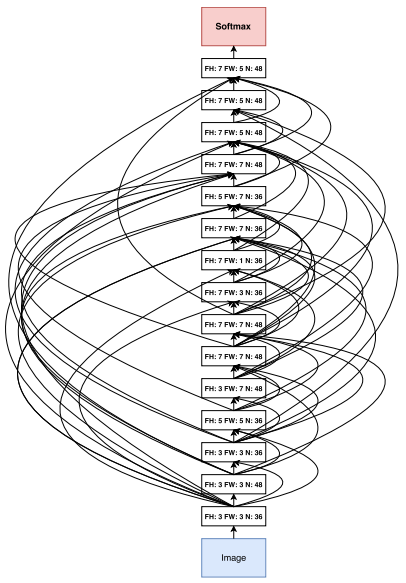
\includegraphics[scale = 0.2]{/home/alex/python/D'yakonov/nas_final1.png} \\

\end{tabular}
\caption{{\footnotesize LSTM и полученные модели: модуль рекуррентной нейросети и архитектура для CIFAR10}}
\end{center}
\end{table}

\end{frame}

\begin{frame}\frametitle{Sim2Real with meta learning}

\begin{block}{{\footnotesize Проблема}}
{\footnotesize 
\begin{itemize}
\item есть задачи, где обучение напрямую либо очень дорого, либо невозможно
\item обучение в сложном симуляторе  вычислительно затратно
\item модель эксплуатирует баги симулятора
\end{itemize} 
}
\end{block}

\begin{block}{{\footnotesize Идея}}
{\footnotesize 
\begin{itemize}
\item рандомизировать параметры симулятора
\end{itemize}
}
{\footnotesize }

\end{block}

\end{frame}

\begin{frame}\frametitle{Sim2Real with meta learning}

\begin{block}{{\footnotesize Метод [Peng et al., 2017]}}
{\footnotesize
\begin{itemize}

\item Промоделируем динамику настоящей среды:  
\begin{center}
$\hat{p}(s_{t+1}|a_t, s_t, \mu) \approx p^*(s_{t+1}|a_t, s_t)$
\end{center} 

\item $\mu$ --- множество параметров(масса конечностей робота, масса и трение шайбы, высота стола и т.д)

\item Задача сводится к оптимизации:
\begin{center}
$ \max \limits_{\pi} E_{\mu \sim \rho_{\mu}} \left[ E_{\tau \sim p(\tau|\pi,\mu)} \left[  \sum \limits_{t=0}^{T-1} r(s_t, a_t) \right] \right]$
\end{center} 

\item Параметры $\mu$ не известны для настоящей среды

\item Научимся оценивать $\mu$ через историю взаимодействия со средой 
\begin{center} $h_t = [a_{t-1}, s_{t-1}, a_{t-2}, s_{t-2}...]$ \end{center} 

\item Для этого наделим policy функцию памятью $\pi(a_t|s_t, z_t)$

\end{itemize}
}
\end{block}

\end{frame}

\begin{frame}\frametitle{Recurrent Deterministic Policy Gradient(RDPG)}

\begin{block}{{\footnotesize Метод [N. Heess et al., 2015]}}
{\footnotesize 
\begin{itemize}
\item Для обучения рекуррентных детерминированных policy функций есть специальный алгоритм.
\item Две обучаемые функции: policy ($\pi(s_t, z_t)$), action-value или omniscient critic ($Q(s_t, a_t, y_t, \mu)$), где $y_t = y(h_t)$ --- внутренняя память
\item Action-value функция: $ Q^{\pi}(s_t,a_t)= E\left[ \sum \limits_{i=t} \gamma^{i-t} r_{i} \;\middle|\; s_t, a_t, \pi\right] $
\item Action-value функция обновляется согласно равенству Беллмана:
\begin{center}
$Q^*(s,a)= E_{s'}\left[  r_t + \gamma \max\limits_{a'} Q^*(s',a') \right]$
\end{center}
\end{itemize}

}
\end{block}

\end{frame}

\begin{frame}\frametitle{Hindsight Experience Replay}
{\footnotesize
\begin{block}{Проблема}

\begin{itemize}
\item Одна из главных проблем в RL --- исследование среды(exploration)
\item Рандомные действия на первых шагах должны приносить награду, иначе нечего учить
\item В случае разреженной функции вознаграждения обучение невозможно
\end{itemize}

\end{block}

\begin{block}{Идея}
\begin{itemize}
\item Построить модель, которая может попасть в любое состояние, не только целевое
\item Например нужно попасть в точку А, попадаем в B, делаем вид что так и надо
\end{itemize}
\end{block}
}
\end{frame}

\begin{frame}\frametitle{Hindsight Experience Replay}

\begin{figure}[h]
\begin{center}
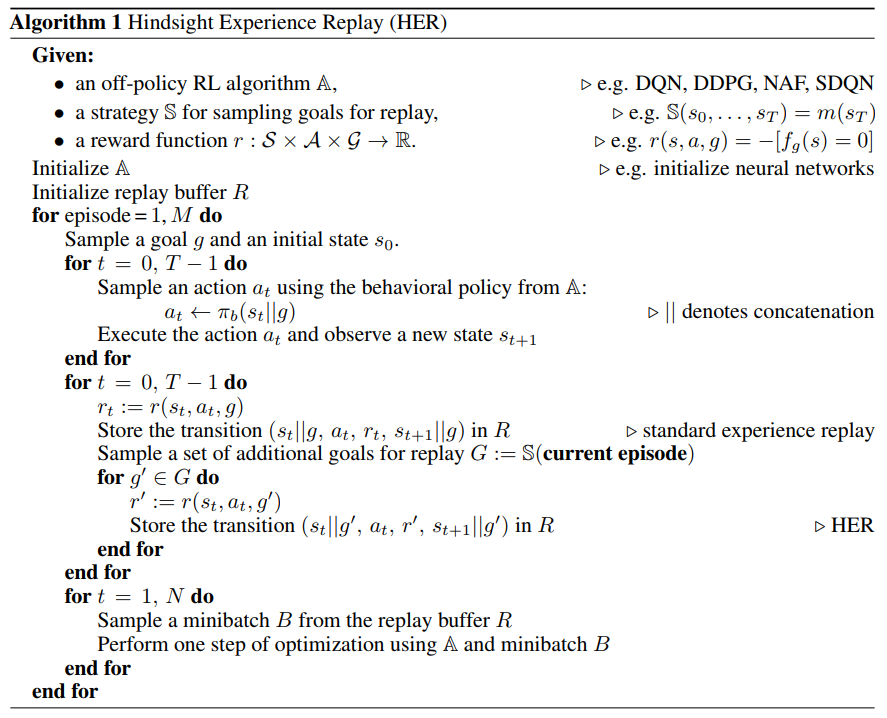
\includegraphics[scale=0.35]{/home/alex/python/D'yakonov/HER.png}
\caption{ Алгоритм, позволяющий справляться с разреженными функциями вознаграждений.}
\end{center}
\end{figure}

\end{frame}


\begin{frame}\frametitle{Hindsight Experience Replay}
\begin{center}
\movie[width=10cm,height=5cm,showcontrols]{}{Hindsight Experience Replay.mp4}
\end{center}
\end{frame}

\begin{frame}\frametitle{Sim2Real with meta learning}

\begin{figure}[h]
\begin{center}
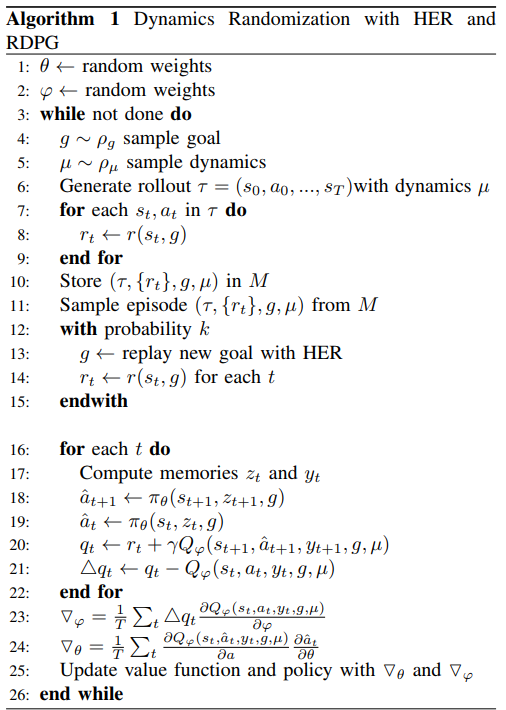
\includegraphics[scale=0.35]{/home/alex/python/D'yakonov/sim2real.png}
\caption{ Основной алгоритм обучения агента}
\end{center}
\end{figure}

\end{frame}

\begin{frame}\frametitle{Sim2Real with meta learning}
\begin{center}
\movie[width=10cm,height=5cm,showcontrols]{}{Sim-to-Real Transfer of Robotic Control with Dynamics Randomization.mp4}
\end{center}
\end{frame}


\begin{frame}\frametitle{Model-Agnostic Meta-Learning for Fast Adaptation of Deep Networks}
{\footnotesize 
\begin{block}{Проблема}
\begin{itemize}
\item Есть задачи с небольшим количеством данных
\item Алгоритм должен уметь быстро, с очень небольшим количеством обучающих примеров, адаптироваться под решение новых задач. \item Например научить классифицировать изображения чайника модель, которая уже умеет классифицировать множество объектов.

\end{itemize}

\end{block}
\begin{block}{Идея}

\begin{itemize}
\item Можно представить задачу следующим образом: модель $f$ работает с множеством задач $T$, из распределения $p(T)$. 
\item Чтобы избежать переобучения и решить новую задачу важно найти параметры модели, сильно влияющие на функции потерь каждой задачи из $p(T)$.
\item Не делается никаких предположений, кроме того, что модель параметризована, данный подход можно обобщить на широкий круг задач от классификации до reinforcement learning. 
\end{itemize}
\end{block}
}
\end{frame}

\begin{frame}\frametitle{Model-Agnostic Meta-Learning for Fast Adaptation of Deep Networks}

\begin{figure}[h]
\begin{center}
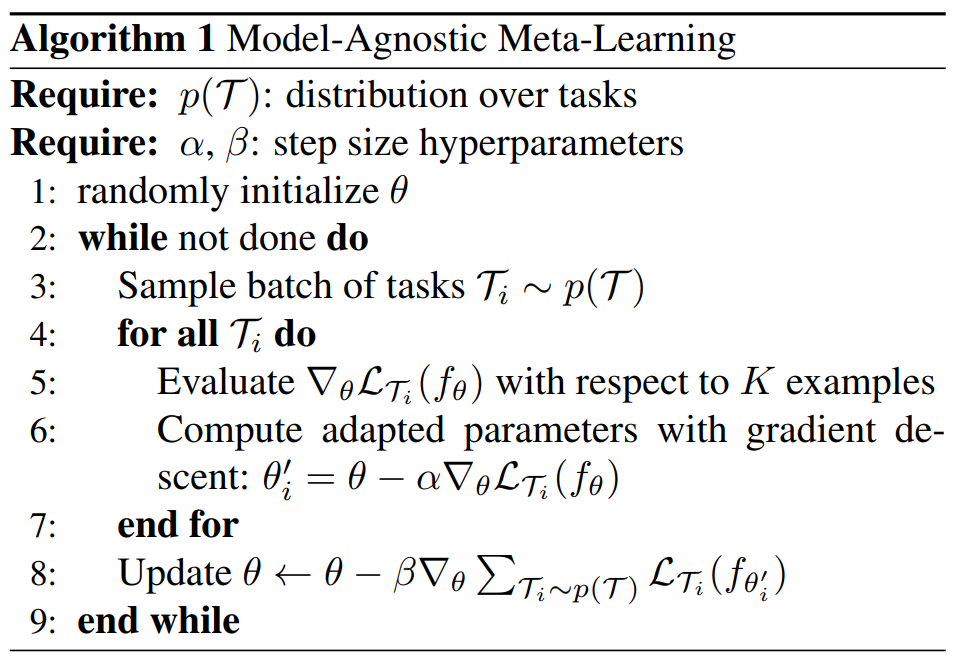
\includegraphics[scale=0.35]{/home/alex/python/D'yakonov/maml.png}
\caption{ Алгоритм MAML в общем виде}
\end{center}
\end{figure}

\end{frame}

\begin{frame}\frametitle{Model-Agnostic Meta-Learning for Fast Adaptation of Deep Networks}

\begin{figure}[h]
\begin{center}
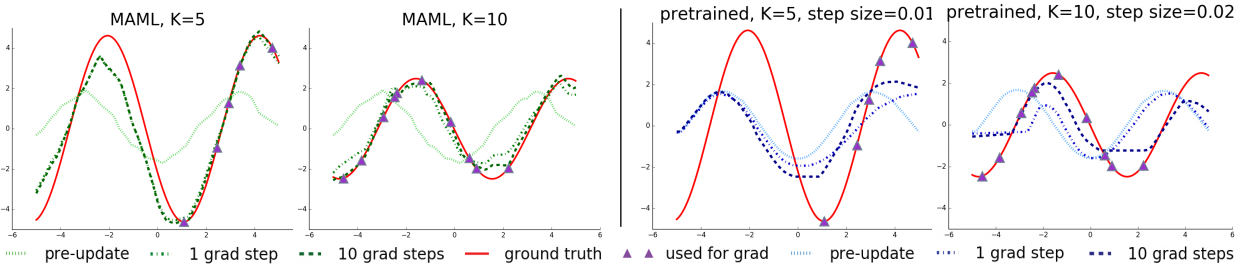
\includegraphics[scale=0.35]{/home/alex/python/D'yakonov/maml_regression.png}
\caption{{\footnotesize  Алгоритм MAML для регрессии}}
\end{center}
\end{figure}

\end{frame}
\begin{frame}\frametitle{Model-Agnostic Meta-Learning for Fast Adaptation of Deep Networks}

\begin{figure}[h]
\begin{center}
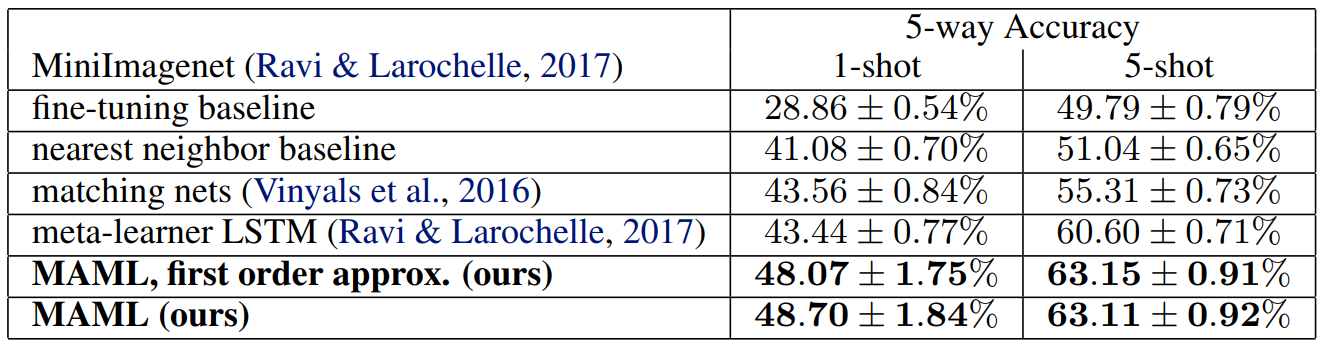
\includegraphics[scale=0.3]{/home/alex/python/D'yakonov/classification.png}
\caption{ Алгоритм MAML для классификации}
\end{center}
\end{figure}

\end{frame}

\begin{frame}\frametitle{Optimization as a model for few-shot learning}

\begin{block}{Идея [Sachin Ravi and Hugo Larochelle, 2017]}
{\footnotesize 
\begin{itemize}
\item Научить модель определять способ обновления параметров конечного алгоритма
\item Формула шага градиентного спуска:
\begin{center}
 $ \theta_t = \theta_{t-1} - \alpha_t \nabla_{\theta_{t-1}}L_t$
\end{center}
\item Формула обновления памяти ячейки LSTM сети (cell state):
\begin{center}
 $ c_t = f_t \odot c_{t-1} + i_t \odot \tilde{c}_t$
\end{center}

\item $c_t$ будет играть роль параметров сети $\theta_t$, $\tilde{c}_t = \nabla_{\theta_{t-1}}L_t$

\item Теперь learning rate зависит от функции потерь, ее градиента, параметров сети и своего значения на предыдущем шаге

\item $i_t = \sigma(W_I \cdot \left[ \nabla_{\theta_{t-1}}L_t, L_t, \theta_{t-1}, i_{t-1} \right] + b_I)$

\item Константа $f_t = 1$ не оптимальна, уменьшение параметров и забывание части предыдущих их значений может оказаться полезным в точке неудачного локального оптимума

\item $f_t = \sigma(W_F \cdot \left[ \nabla_{\theta_{t-1}}L_t, L_t, \theta_{t-1}, f_{t-1} \right] + b_F)$

\end{itemize}

}
\end{block}

\end{frame}

\begin{frame}\frametitle{Optimization as a model for few-shot learning}
\begin{figure}[h]
\begin{center}
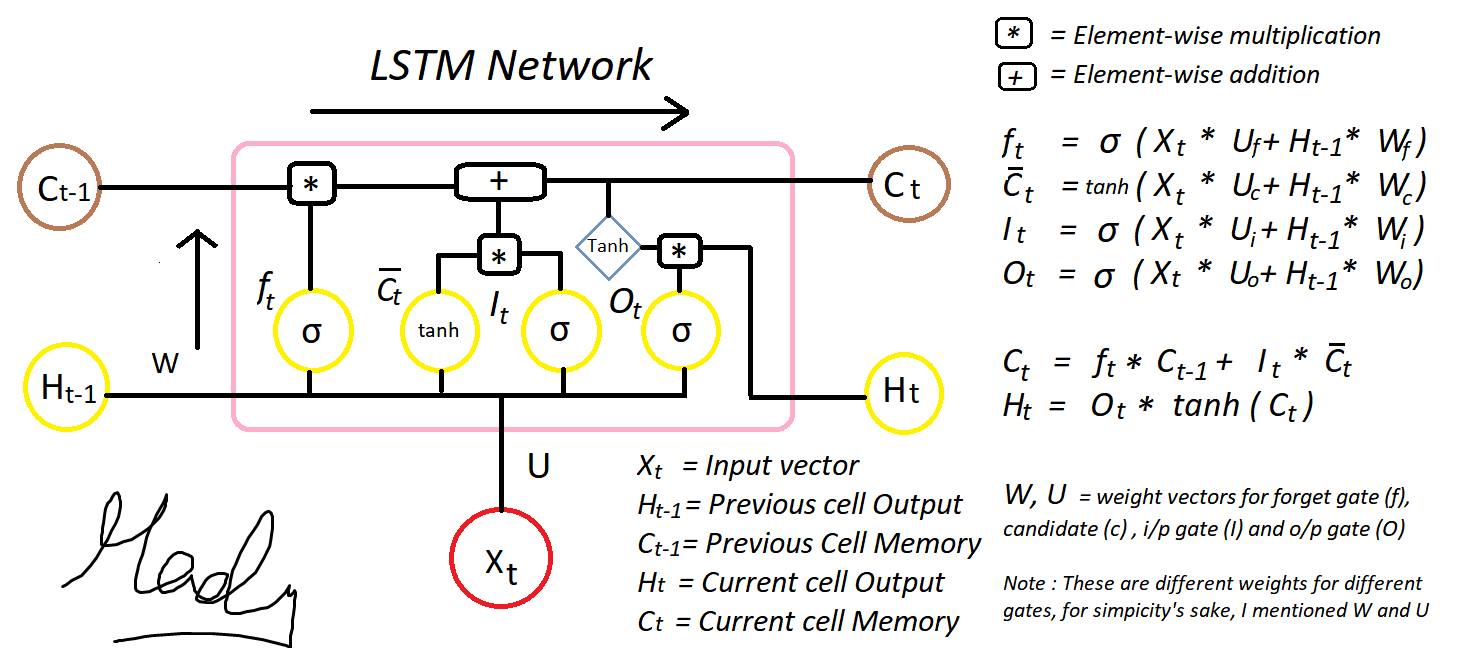
\includegraphics[scale=0.2]{/home/alex/python/D'yakonov/LSTM_explained.png}
\caption{{\footnotesize Архитектура LSTM }}
\end{center}
\end{figure}
\end{frame}


\begin{frame}\frametitle{Optimization as a model for few-shot learning}
\begin{figure}[h]
\begin{center}
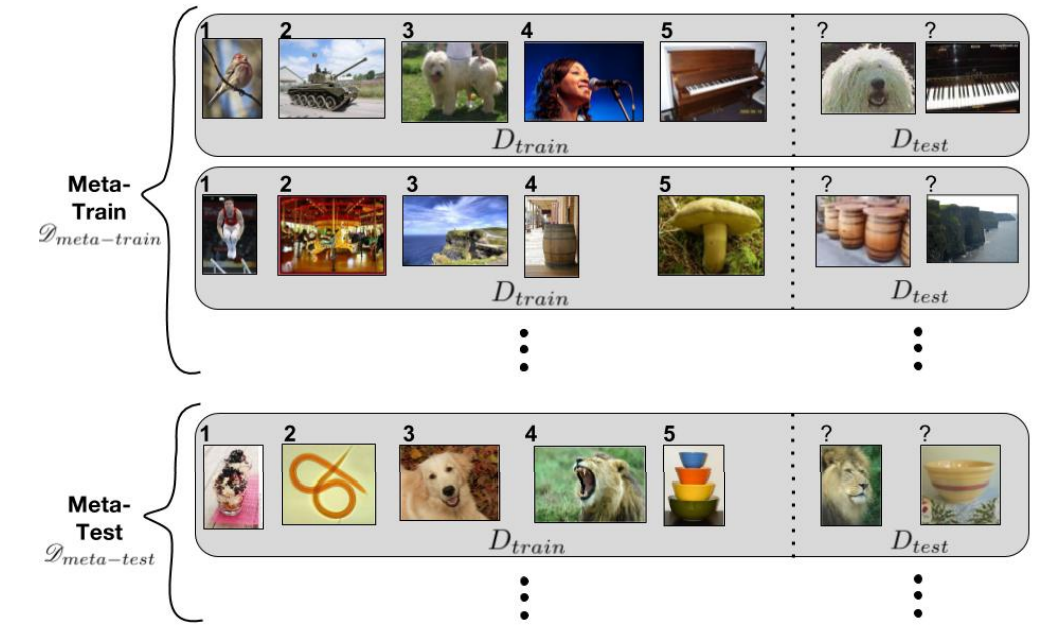
\includegraphics[scale=0.3]{/home/alex/python/D'yakonov/lstm_meta_sets.png}
\caption{{\footnotesize Обучение Meta-Learner'а происходит на множестве пар датасетов, называемых эпизодами. Каждая пара состоит из тренировочной и тестовой выборки. В тренировочной выборке присутствуют k*N элементов, где N --- количество классов, а k --- ограничение на количество элементов из одного класса. }}
\end{center}
\end{figure}
\end{frame}

\begin{frame}\frametitle{Optimization as a model for few-shot learning}

\begin{figure}[h]
\begin{center}
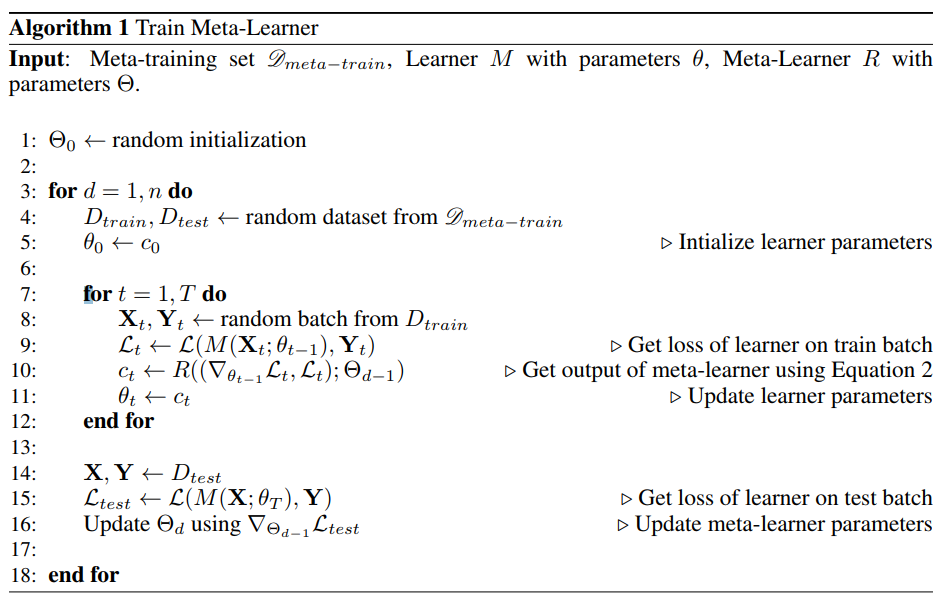
\includegraphics[scale=0.35]{/home/alex/python/D'yakonov/lstm_meta_alg.png}
\caption{{\footnotesize  Алгоритм обучения Meta-Learner}}
\end{center}
\end{figure}

\end{frame}

\begin{frame}\frametitle{Optimization as a model for few-shot learning}
\begin{figure}[h]
\begin{center}
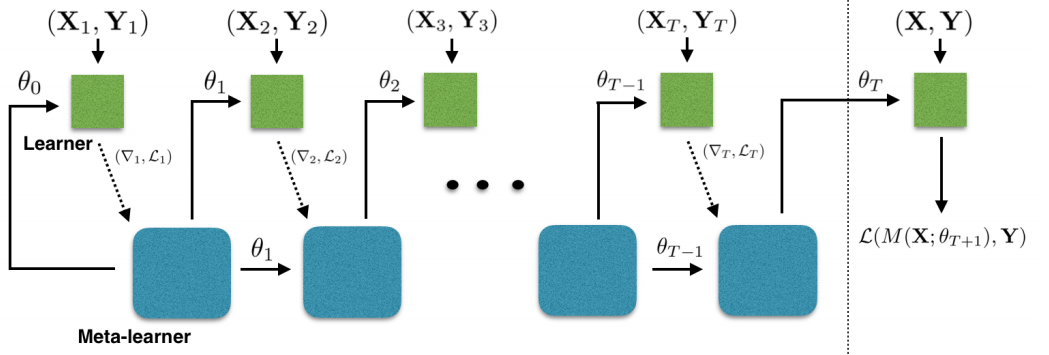
\includegraphics[scale=0.4]{/home/alex/python/D'yakonov/lstm_meta_simpl.png}
\caption{{\footnotesize  Проход вперед(forward pass) meta learner'a. Как видно часть стрелок пунктирные, это означает, что во время обновления весов эти шаги не учитываются. Это позволяет избежать появления вторых производных и сильно упрощает вычисления. Пунктирной линией отделены шаги на тестовой и тренировочной выборках.}}
\end{center}
\end{figure}
\end{frame}

\begin{frame}\frametitle{Limitations of meta learning}
{\footnotesize
\begin{block}{Ограничения}
\begin{itemize}
\item Распределение задач на тренировочной выборке должно быть тем же что и на тестовой
\item Пример случая, когда новая задача \textbf{фундаментально} отличается от тренировочных: если мы обучим модель математике, программированию, чтению и т.д. сможет ли модель в результате выучить химию?

\end{itemize}
\end{block}
}
\end{frame}

\begin{frame}\frametitle{References}
{\footnotesize  
\begin{itemize}
\item N. Heess, J. J. Hunt, T. P. Lillicrap, and D. Silver, <<Memory-based
control with recurrent neural networks>>, http://arxiv.org/abs/1512.04455
\item Barret Zoph, Quoc V. Le, <<Neural Architecture Search>>, https://openreview.net/pdf?id=r1Ue8Hcxg
\item Marcin Andrychowicz, Filip Wolski, Alex Ray, Jonas Schneider, Rachel Fong,
Peter Welinder, Bob McGrew, Josh Tobin, Pieter Abbeel
, Wojciech Zaremba, <<Hindsight Experience Replay>>, https://arxiv.org/pdf/1707.01495v3.pdf
\item Chelsea Finn, Pieter Abbeel, Sergey Levine, <<Model-Agnostic Meta-Learning for Fast Adaptation of Deep Networks>>, https://arxiv.org/pdf/1703.03400.pdf
\item Sachin Ravi, Hugo Larochelle, <<Optimization as a model for few-shot learning>>, https://openreview.net/pdf?id=rJY0-Kcll
\item Xue Bin Peng, Marcin Andrychowicz, Wojciech Zaremba, Pieter Abbeel1, <<Sim-to-Real Transfer of Robotic Control with Dynamics Randomization>>, https://arxiv.org/pdf/1710.06537.pdf
\end{itemize}

}

\end{frame}
\end{document}

